\chapter{Részletes tervezés}
\label{chap:tervezes}

Ebben a fejezetben a rendszer konkrét tervezési döntéseit mutatom be. A specifikációs fejezetben meghatározott követelmények után itt már az a kérdés, hogyan épül fel a saját adathalmaz, milyen jellemzőket érdemes kinyerni a hangból, hogyan készülnek a kísérleti adathalmazok, és milyen modellarchitektúra illeszkedik ehhez a feladathoz.

A fejezet nem minden egyes segédfüggvény dokumentációja. Inkább azt a mérnöki gondolatmenetet követi végig, amely elvezetett a végső Log-Mel + 2D CNN pipeline-hoz, valamint a YAMNet transfer learning összehasonlító modellhez.

%% ═══════════════════════════════════════════════════════════════════════════
\section{Az adathalmaz tervezése}
\label{sec:dataset_design}

A hangszerfelismerési feladatban az adathalmaz minősége legalább annyira meghatározó, mint maga a neurális hálózat. A célom nem egy nagyon nagy, de nehezen átlátható adathalmaz létrehozása volt, hanem egy kisebb, kontrollált, kísérletezésre alkalmas adatbázis, amelyben a tiszta, augmentált és mikrofonos változatok szerepe elkülöníthető.

Az osztályrendszert hét kategóriára bontottam:
\begin{enumerate}
  \item[(1)] Gitár: akusztikus és kevésbé torzított elektromos gitárok,
  \item[(2)] Zongora: klasszikus és digitális zongorahangok,
  \item[(3)] Vokál: énekhang és néhány karakteres emberi hangképzés,
  \item[(4)] Vonós: hegedű, brácsa, cselló, nagybőgő,
  \item[(5)] Nádfúvós: klarinét, szaxofon, oboa, fagott,
  \item[(6)] Rézfúvós: trombita, harsona, kürt, tuba,
  \item[(7)] Zaj/csend: környezeti zajok, háttérzajok és csendközeli szakaszok.
\end{enumerate}

Ez a kategóriarendszer tudatos kompromisszum. A rövid, 1 másodperces mintákon belül egyes konkrét hangszerek nagyon hasonló akusztikai jegyeket hordoznak, ezért a hangszercsalád-szintű felismerés stabilabb és a valós idejű demonstrációhoz is jobban illeszkedik.

\subsection{A forrásadatok kiválasztása}
\label{subsec:own_dataset}

A tervezés elején megvizsgáltam néhány ismert publikus adathalmazt, mert ezek jól mutatják, milyen irányok léteznek a hangszerfelismerésben. A cél végül nem ezek összeolvasztása lett, hanem egy saját, a dolgozat céljához igazított organikus adathalmaz létrehozása. A vizsgált források legfontosabb tanulságait a \ref{tab:adathalmaz_osszehasonlitas}.~táblázat foglalja össze.

\begin{table}[H]
\centering
\caption{A vizsgált publikus adathalmazok tervezési szempontú összefoglalása}
\label{tab:adathalmaz_osszehasonlitas}
\resizebox{\textwidth}{!}{%
\begin{tabular}{p{2.4cm}p{4.2cm}p{4.5cm}p{4.4cm}}
\toprule
\textbf{Adathalmaz} & \textbf{Tartalom} & \textbf{Hasznos tanulság} & \textbf{Korlát ebben a projektben} \\
\midrule
\textbf{IRMAS}~\cite{bosch2012irmas} & Valós zenei részletek szóló hangszeres jelöléssel & Jó példa valós zenei környezetre & Eltérő kategóriarendszer és korlátozott egyensúly \\
\textbf{NSynth}~\cite{engel2017nsynth} & Nagy mennyiségű izolált hangszerhang & Egységes, kontrollált minták & Túl steril; nem folytonos zenei részletek \\
\textbf{TinySOL}~\cite{cella2020tinysol} & Izolált zenekari hangszerek & Jó minőségű referenciahangok & Kevésbé reprezentálja a valós előadást \\
\textbf{Good-sounds}~\cite{romani2015good} & Fúvós és vonós hangjegyek & Változatos felvételi minőségek & Hiányzik több célosztály, például gitár és vokál \\
\textbf{ESC-50}~\cite{piczak2015esc} & Környezeti hangok és zajok & Kiváló zaj/csend kategóriához & Nem tartalmaz hangszeres osztályokat \\
\bottomrule
\end{tabular}%
}
\end{table}

A végső döntés az lett, hogy a hangszeres osztályokhoz interneten elérhető zenei felvételekből válogatok karakteres, többnyire jól felismerhető részleteket, a zaj/csend osztályt pedig az ESC-50 adathalmazból egészítem ki. Az internetes hangmintákat kizárólag oktatási és kutatási célra használom, a nyers forrásfájlokat nem teszem közzé és nem terjesztem.

\subsection{Felosztás és leakage-csökkentés}

A felosztásnál a legfontosabb tervezési kockázat az adatszivárgás volt. Ha először 1 másodperces szeleteket hoznék létre, és csak ezután osztanám szét őket train, validation és test halmazba, akkor ugyanannak az 5 másodperces zenei blokknak nagyon hasonló részletei több halmazba is bekerülhetnének. Ez túl optimista validációs eredményt adna.

Ezért a \texttt{01\_prepare\_\allowbreak clean\_\allowbreak dataset.py} először az 5 másodperces blokkokat osztja szét rétegzett, osztályonként kiegyensúlyozott módon, nagyjából 70\%/15\%/15\% arányban. Az 1 másodperces szeletelés csak ezután történik meg. Így az egy blokkból származó szeletek azonos halmazban maradnak. Forrásfelvétel-szintű teljes szeparációt a kis adatmennyiség miatt nem állítok, de a szeletek közötti közvetlen leakage kockázatát ezzel a megoldással jelentősen csökkentettem.

Az első, tiszta adathalmaz hozzávetőleges eloszlását a \ref{fig:organic_class_distribution}.~ábra szemlélteti.

\begin{figure}[H]
\centering
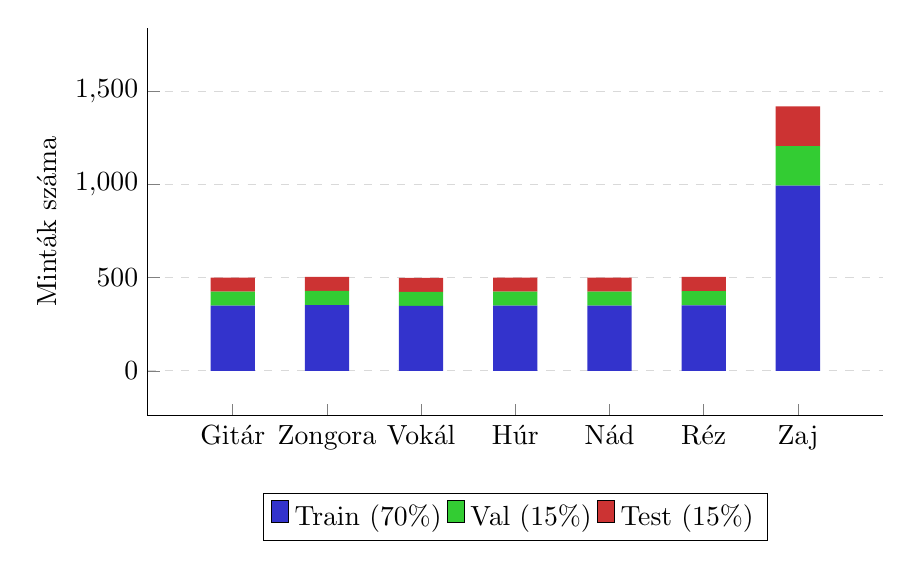
\begin{tikzpicture}
\begin{axis}[
    ybar stacked,
    bar width=16pt,
    enlargelimits=0.15,
    ylabel={Minták száma},
    symbolic x coords={Gitár, Zongora, Vokál, Húr, Nád, Réz, Zaj},
    xtick=data,
    ymin=0,
    ymax=1600,
    width=0.9\textwidth,
    height=6.5cm,
    axis x line*=bottom,
    axis y line*=left,
    ymajorgrids=true,
    grid style={dashed, gray!30},
    legend style={at={(0.5,-0.2)}, anchor=north, legend columns=-1},
]
\addplot[fill=blue!60!gray, draw=none] coordinates {
    (Gitár,350) (Zongora,353) (Vokál,349) (Húr,350) (Nád,350) (Réz,352) (Zaj,994)
};
\addplot[fill=green!60!gray, draw=none] coordinates {
    (Gitár,75) (Zongora,76) (Vokál,75) (Húr,75) (Nád,75) (Réz,76) (Zaj,213)
};
\addplot[fill=red!60!gray, draw=none] coordinates {
    (Gitár,75) (Zongora,76) (Vokál,75) (Húr,75) (Nád,75) (Réz,76) (Zaj,213)
};
\legend{Train (70\%), Val (15\%), Test (15\%)}
\end{axis}
\end{tikzpicture}
\caption{A saját gyűjtésű tiszta adathalmaz hozzávetőleges eloszlása a szeparált szeletelés után}
\label{fig:organic_class_distribution}
\end{figure}

\subsection{Mikrofonos újrafelvétel}
\label{subsec:mic_recording}

A projekt egyik fontos célja a valós idejű, mikrofonos felismerés. Emiatt a tiszta internetes minták önmagukban nem elegendőek, mert nem tartalmazzák a saját laptopmikrofon, a szoba és a visszajátszó eszköz hatását. Ezt a különbséget domain shiftnek tekintem, és külön kísérleti adathalmazokkal mérem.

A mikrofonos adatok előállításához nem egyenként játszottam fel minden mintát, hanem automatizált folyamatot terveztem. A \texttt{02\_acquire\_\allowbreak mic\_\allowbreak data.py} split és osztály szerint összefűzi a tiszta mintákat, a hanganyag elejére szinkronizációs sípszót tesz, majd a telefonról visszajátszott jelet a laptop beépített mikrofonjával rögzíti. A script a sípszó alapján újraigazítja a felvételt, és visszaszeleteli 1 másodperces mintákra.

\begin{figure}[H]
\centering
\begin{tikzpicture}[
    node distance=1.0cm and 0.7cm,
    block/.style={draw, rectangle, minimum height=1.3cm, minimum width=2.5cm, fill=blue!5!white, text width=2.3cm, align=center, font=\footnotesize, rounded corners},
    arrow/.style={thick,->,>=stealth}
]
\node (orig) [block] {Tiszta split minták};
\node (concat) [block, right=of orig] {Összefűzés sípszóval};
\node (play) [block, right=of concat] {Telefonos lejátszás};
\node (record) [block, below=of play] {Laptop mikrofonos rögzítés};
\node (sync) [block, left=of record] {Szinkronizáció};
\node (slice) [block, left=of sync] {Szeletelés és rendezés};

\draw [arrow] (orig) -- (concat);
\draw [arrow] (concat) -- (play);
\draw [arrow] (play) -- (record);
\draw [arrow] (record) -- (sync);
\draw [arrow] (sync) -- (slice);
\end{tikzpicture}
\caption{A mikrofonos újrafelvételi és szinkronizált szeletelési folyamat}
\label{fig:mic_recording_pipeline}
\end{figure}

A mikrofonos train, validation és test változatok szerepe elkülönül. A mikrofonos train minták csak a végső modell tanításába kerülnek be, míg a mikrofonos validation és test minták a célkörnyezet mérésére szolgálnak. Így nem tanítok rá a kiértékelési mintákra, de mégis meg tudom mérni, mennyit változik a teljesítmény a mikrofonos domainben.

A kísérleti adathalmazok egy osztályra vetített, kerekített felépítését a \ref{fig:mic_recorded_distribution}.~ábra mutatja.

\begin{figure}[H]
\centering
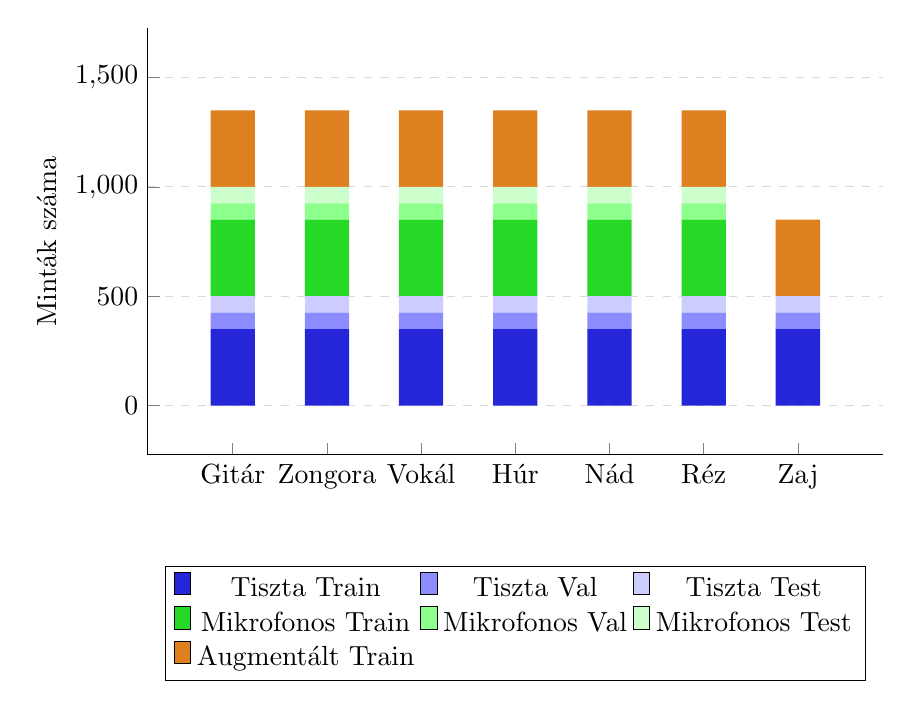
\begin{tikzpicture}
\begin{axis}[
    ybar stacked,
    bar width=16pt,
    enlargelimits=0.15,
    ylabel={Minták száma},
    symbolic x coords={Gitár, Zongora, Vokál, Húr, Nád, Réz, Zaj},
    xtick=data,
    ymin=0,
    ymax=1500,
    width=0.9\textwidth,
    height=7cm,
    axis x line*=bottom,
    axis y line*=left,
    ymajorgrids=true,
    grid style={dashed, gray!30},
    legend style={at={(0.5,-0.26)}, anchor=north, legend columns=3},
]
\addplot[fill=blue!70!gray, draw=none] coordinates {
    (Gitár,350) (Zongora,350) (Vokál,350) (Húr,350) (Nád,350) (Réz,350) (Zaj,350)
};
\addplot[fill=blue!45!white, draw=none] coordinates {
    (Gitár,75) (Zongora,75) (Vokál,75) (Húr,75) (Nád,75) (Réz,75) (Zaj,75)
};
\addplot[fill=blue!20!white, draw=none] coordinates {
    (Gitár,75) (Zongora,75) (Vokál,75) (Húr,75) (Nád,75) (Réz,75) (Zaj,75)
};
\addplot[fill=green!70!gray, draw=none] coordinates {
    (Gitár,350) (Zongora,350) (Vokál,350) (Húr,350) (Nád,350) (Réz,350) (Zaj,0)
};
\addplot[fill=green!45!white, draw=none] coordinates {
    (Gitár,75) (Zongora,75) (Vokál,75) (Húr,75) (Nád,75) (Réz,75) (Zaj,0)
};
\addplot[fill=green!20!white, draw=none] coordinates {
    (Gitár,75) (Zongora,75) (Vokál,75) (Húr,75) (Nád,75) (Réz,75) (Zaj,0)
};
\addplot[fill=orange!75!gray, draw=none] coordinates {
    (Gitár,350) (Zongora,350) (Vokál,350) (Húr,350) (Nád,350) (Réz,350) (Zaj,350)
};
\legend{Tiszta Train, Tiszta Val, Tiszta Test, Mikrofonos Train, Mikrofonos Val, Mikrofonos Test, Augmentált Train}
\end{axis}
\end{tikzpicture}
\caption{A kísérleti adathalmazok hozzávetőleges felépítése osztályonként, kerekített mintaszámokkal}
\label{fig:mic_recorded_distribution}
\end{figure}

\subsection{A négy kísérleti adathalmaz}
\label{subsec:final_dataset}

A végső adatfolyam nem egyetlen nagy adathalmazt hoz létre, hanem négy elkülönített kísérleti változatot az \texttt{experiment\_datasets/} könyvtárban. Ezekből a \texttt{04a\_extract\_\allowbreak features.py} script készíti el a tanításhoz használt NumPy tömböket a \texttt{processed\_data/} könyvtár alatt.

\begin{table}[H]
\centering
\caption{A végleges kísérleti adathalmazok tényleges mérete}
\label{tab:final_dataset_counts}
\begin{tabular}{lrrr}
\toprule
\textbf{Adathalmaz} & \textbf{Train} & \textbf{Validation} & \textbf{Test} \\
\midrule
\texttt{exp\_clean} & 2420 & 542 & 536 \\
\texttt{exp\_augmented} & 4841 & 542 & 536 \\
\texttt{exp\_naive\_deployment} & 4841 & 562 & 557 \\
\texttt{exp\_final} & 7278 & 562 & 557 \\
\bottomrule
\end{tabular}
\end{table}

Az \texttt{exp\_clean} az alap tiszta mérés, az \texttt{exp\_augmented} a szoftveres augmentáció hatását mutatja, az \texttt{exp\_naive\_deployment} a mikrofonos célkörnyezet okozta visszaesést méri, az \texttt{exp\_final} pedig a végső, mikrofonos train adatokkal is megerősített rendszert képviseli. A validációs és teszthalmaz szerepe itt is elkülönül: validáció alapján választok modellt, a test csak a kiválasztott végső modellek ellenőrzésére szolgál.

%% ═══════════════════════════════════════════════════════════════════════════
\section{Jellemzőkinyerés tervezése}
\label{sec:feature_extraction}

A nyers hullámforma közvetlenül is használható mélytanulási bemenetként, de a saját 2D CNN modellhez célszerűbb idő-frekvencia reprezentációt készíteni. A tervezés során három, szakmailag jól elkülöníthető jellemzőtípust vizsgáltam:
\begin{itemize}
  \item \textbf{STFT spektrogram:} lineáris frekvenciaskálájú, közvetlen idő-frekvencia ábrázolás;
  \item \textbf{MFCC:} klasszikus, tömörített, kepsztrális audio baseline;
  \item \textbf{Log-Mel spektrogram:} perceptuális, képszerű reprezentáció, amely jól illeszkedik a 2D CNN-hez.
\end{itemize}

Nem az volt a célom, hogy minden lehetséges zenei jellemzőt kipróbáljak. A chroma, tonnetz vagy spectral contrast inkább hangmagassági és harmóniai jellegű feladatokban hasznos, míg itt rövid minták hangszercsalád-szintű osztályozása a cél. Az STFT--MFCC--Log-Mel hármas ezért elég széles összehasonlítási alapot ad: nyersebb spektrum, klasszikus tömörítés és perceptuális spektrogram.

A használt közös beállítások:
\begin{itemize}
  \item mintavételi frekvencia: $SR = 16\,000$ Hz,
  \item FFT ablakméret: $n\_fft = 1024$,
  \item Log-Mel hop length: $256$ minta,
  \item STFT és MFCC összehasonlító hop length: $512$ minta.
\end{itemize}

\subsection{A három reprezentáció}

\textbf{STFT.} Az STFT decibelre konvertált magnitúdó-spektrogramot ad, $513 \times 32$ méretben. Előnye, hogy megtartja a teljes lineáris frekvenciatengelyt, hátránya viszont a nagyobb bemeneti méret és a kevésbé perceptuális frekvenciafelbontás.

\textbf{MFCC.} Az MFCC-t 40 együtthatóval számolom, így a bemenet $40 \times 32$ méretű. Ez nagyon kompakt reprezentáció, de a diszkrét koszinusz transzformáció miatt eldobhat olyan spektrális finomszerkezeteket, amelyek a hangszerek hangszínéhez fontosak.

\textbf{Log-Mel.} A Log-Mel spektrogram 128 Mel-sávot használ, a finomabb hop length miatt pedig $128 \times 63$ méretű mátrixot ad. Ez lett a saját modell fő bemenete, mert a hangszínt hordozó spektrális szerkezetet még jól megtartja, miközben a bemenet kezelhető méretű marad.

\subsection{A megfelelő jellemzőkinyerési eljárás kiválasztása}
\label{subsec:feature_selection}

A döntést két szempont vezette. Egyrészt a Log-Mel elméletileg is illeszkedik a hallásközeli, képszerű reprezentációhoz; másrészt a clean baseline kísérletekben ez bizonyult a legerősebb saját CNN bemenetnek. Emiatt a későbbi augmentációs, domain shift és final kísérleteket már Log-Mel bemenettel futtattam.

\begin{table}[H]
  \centering
  \caption{A három vizsgált jellemzőkinyerési módszer tervezési összehasonlítása}
  \label{tab:feature_comparison_properties}
  \resizebox{\textwidth}{!}{%
  \begin{tabular}{lllp{4.4cm}p{4.5cm}}
    \toprule
    \textbf{Jellemző} & \textbf{Dimenzió} & \textbf{Skála} & \textbf{Fő előny} & \textbf{Fő korlát} \\
    \midrule
    STFT & $513 \times 32$ & Lineáris & Megőrzi a teljes spektrális szerkezetet. & Nagyobb bemenet, sok magas frekvenciás részlet. \\
    Log-Mel & $128 \times 63$ & Mel-skála & Hallásközeli, CNN-hez jól illeszkedő reprezentáció. & A Mel-sűrítés enyhe információvesztést okoz. \\
    MFCC & $40 \times 32$ & Kepsztrális & Nagyon kompakt klasszikus baseline. & Kevésbé őrzi meg a felharmonikus mintázatot. \\
    \bottomrule
  \end{tabular}%
  }
\end{table}

\begin{figure}[H]
  \centering
  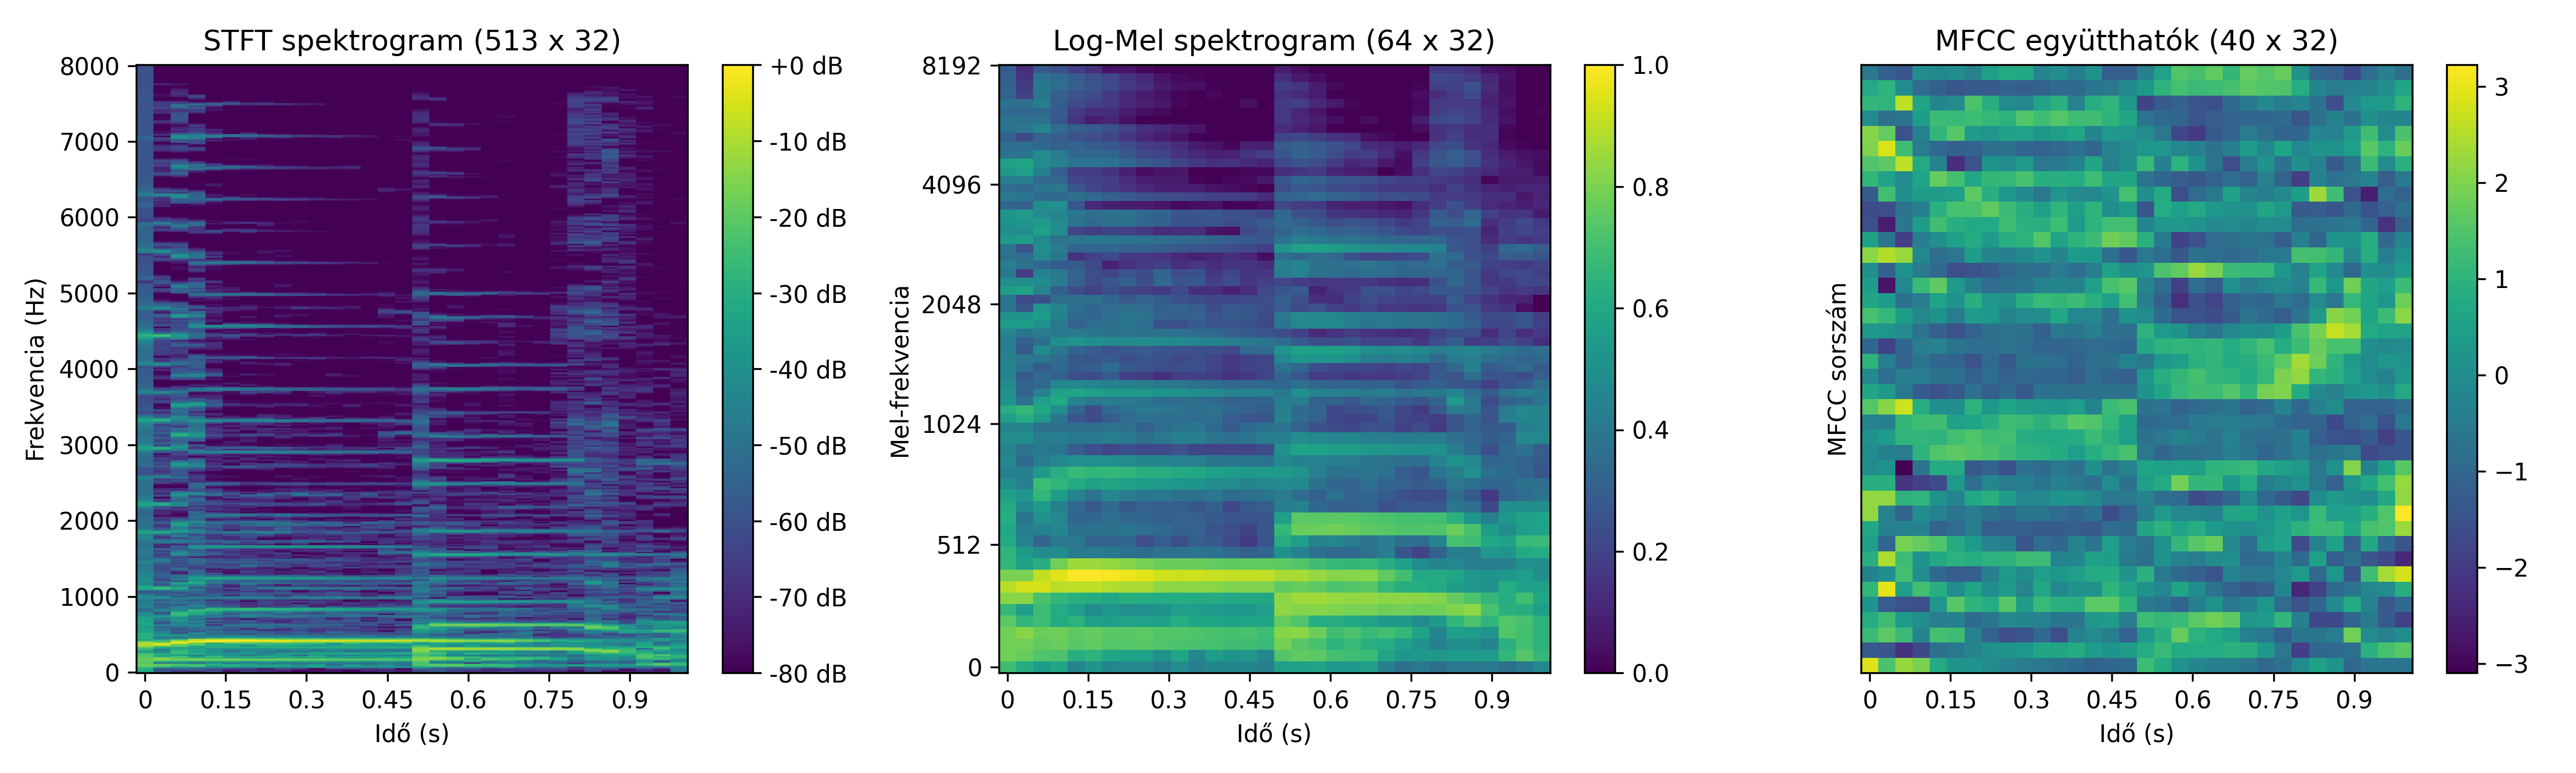
\includegraphics[width=\textwidth]{fig_feature_comparison.png}
  \caption{A projektben összehasonlított három jellemzőtípus ugyanazon gitárminta esetén: STFT, normalizált Log-Mel és normalizált MFCC}
  \label{fig:feature_comparison}
\end{figure}

\subsection{Normalizálás és kimeneti állományok}
\label{subsec:feature_outputs}

A Log-Mel és STFT jellemzőket decibel skálára alakítom, majd a tanítás és a valós idejű felismerés között konzisztens módon $[0,1]$ tartományra skálázom. Az MFCC esetében sávonkénti standardizálást használok. A lényeg az, hogy a modell ugyanabban az értéktartományban kapjon bemenetet tanításkor és inferencia közben.

A kinyert tömbök a \texttt{processed\_data/} könyvtár alá kerülnek, kísérleti adathalmazonként külön mappába. A Log-Mel minden kísérlethez elkészül, az STFT és MFCC csak a clean baseline feature-összehasonlításhoz szükséges, a nyers hanghullám pedig az \texttt{exp\_final} YAMNet transfer learning méréséhez készül el.

%% ═══════════════════════════════════════════════════════════════════════════
\section{Adatbővítés tervezése}
\label{sec:augmentation}

A szoftveres augmentáció célja az volt, hogy a tiszta train minták mellé olyan torzított változatok kerüljenek, amelyek valamennyire hasonlítanak egy fogyasztói eszközön visszajátszott és laptopmikrofonnal rögzített hanghoz. Az augmentáció csak a tanítóhalmazon történik; a validációs és teszthalmazt nem torzítom utólag.

Az augmentációs lánc fő elemei:
\begin{itemize}
  \item \textbf{szobai visszhang:} egyszerű FIR alapú reverb, véletlenszerű késleltetésekkel és csillapítással;
  \item \textbf{pre-emphasis:} a mikrofon és a szoba frekvenciaválaszának durva közelítése;
  \item \textbf{zajkeverés:} ESC-50-ből választott háttérzaj hozzáadása 5--15 dB SNR tartományban;
  \item \textbf{soft clipping:} enyhe nemlineáris torzítás a mikrofonbemenet telítődésének szimulálására;
  \item \textbf{csúcs-normalizálás:} az amplitúdó kontrollált tartományban tartása.
\end{itemize}

\begin{figure}[H]
\centering
\begin{tikzpicture}[
    node distance=1.0cm and 0.8cm,
    block/.style={draw, rectangle, minimum height=1.1cm, minimum width=2.6cm, fill=blue!5!white, text width=2.5cm, align=center, font=\footnotesize, rounded corners},
    arrow/.style={thick,->,>=stealth}
]
  \node (orig) [block] {Tiszta hangszerminta};
  \node (reverb) [block, right=of orig] {Szobai reverb};
  \node (preemph) [block, right=of reverb] {Pre-emphasis};
  \node (noise) [block, right=of preemph] {Zajkeverés};
  \node (clip) [block, below=of noise] {Soft clipping};
  \node (norm) [block, left=of clip] {Normalizálás};
  \node (aug) [block, left=of norm] {Augmentált minta};

  \draw [arrow] (orig) -- (reverb);
  \draw [arrow] (reverb) -- (preemph);
  \draw [arrow] (preemph) -- (noise);
  \draw [arrow] (noise) -- (clip);
  \draw [arrow] (clip) -- (norm);
  \draw [arrow] (norm) -- (aug);
\end{tikzpicture}
\caption{A MacBook/mikrofonos felvételi körülményeket közelítő adataugmentációs lánc}
\label{fig:augmentation_chain}
\end{figure}

\begin{figure}[H]
  \centering
  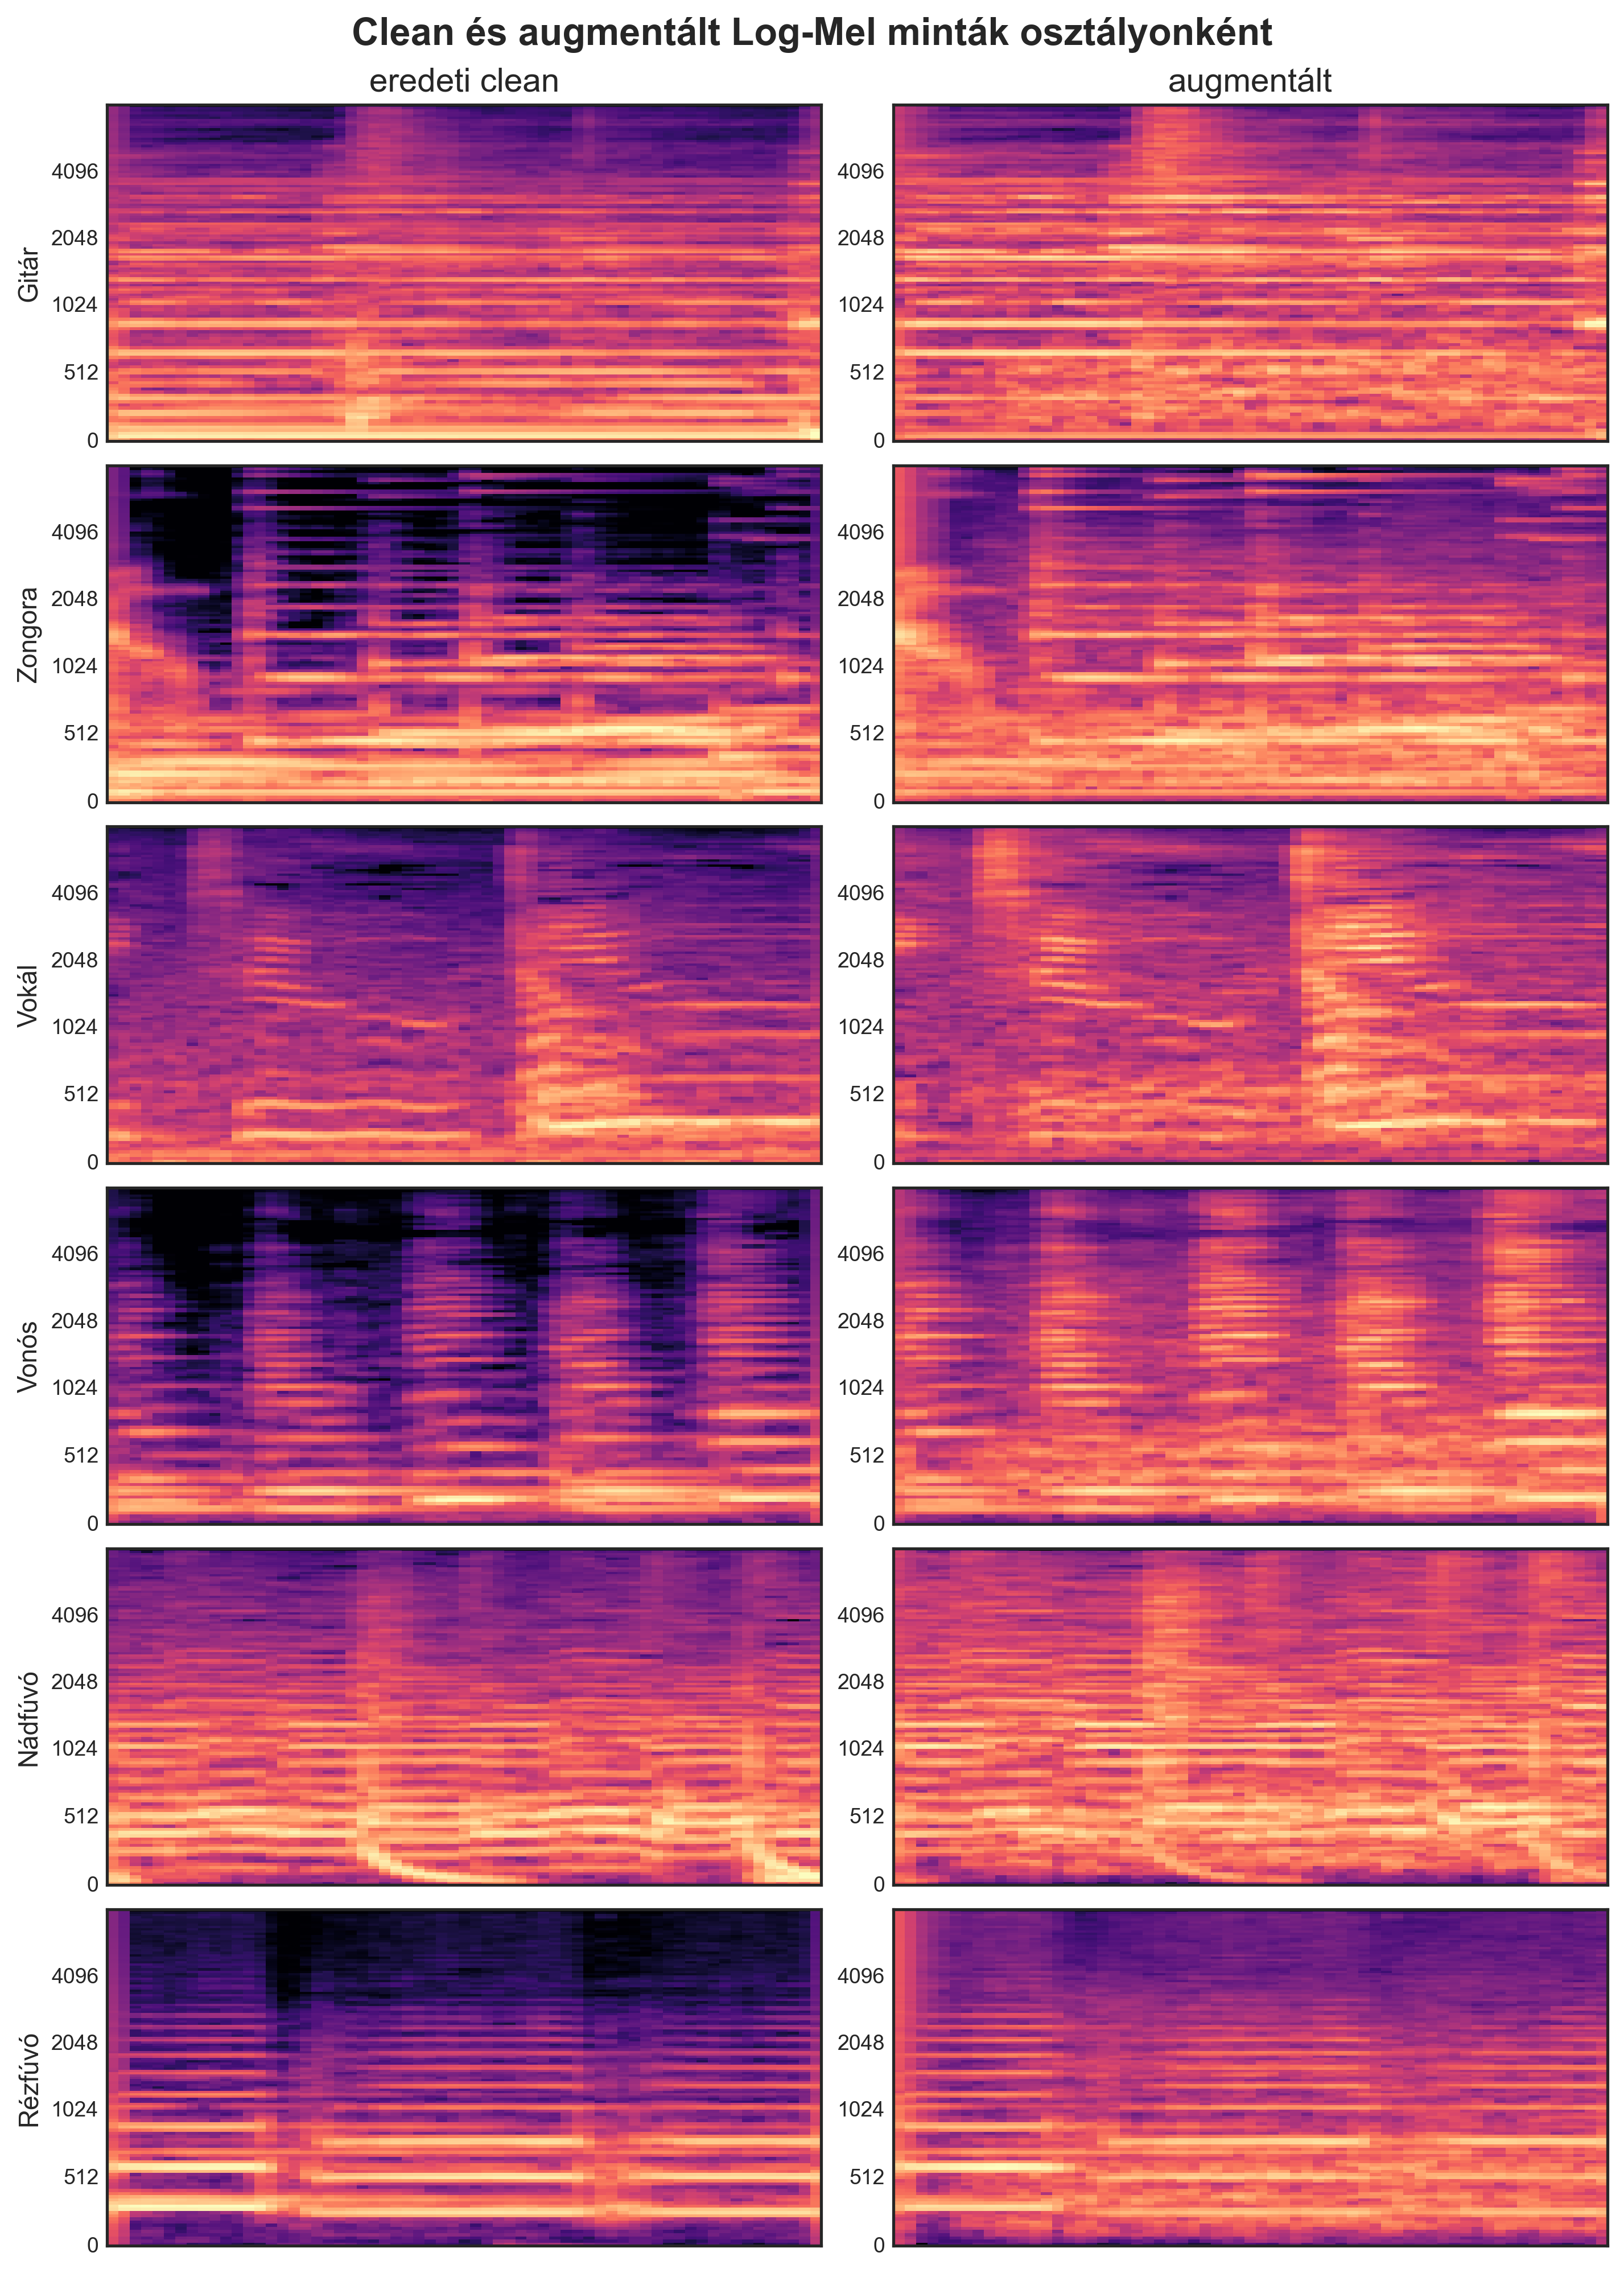
\includegraphics[height=0.72\textheight,keepaspectratio]{fig_original_vs_augmented.png}
  \caption{Reprezentatív minták normalizált Log-Mel spektrogramjai eredeti és augmentált állapotban}
  \label{fig:original_vs_augmented}
\end{figure}

Az augmentáció nem a valós mikrofonos felvétel tökéletes helyettesítése. Inkább egy olcsó és jól kontrollálható regularizációs eszköz, amely segít abban, hogy a modell ne csak steril, tiszta spektrális mintázatokra tanuljon rá.

%% ═══════════════════════════════════════════════════════════════════════════
\section{Modellarchitektúrák tervezése}
\label{sec:cnn_architecture}

A saját rendszer fő modellje egy Log-Mel spektrogramot feldolgozó 2D konvolúciós neurális hálózat. A választás oka nem az volt, hogy minden lehetséges klasszikus és neurális modellváltozatot kimerítően összehasonlítsak, hanem hogy a bemenethez illeszkedő, magyarázható és valós időben is futtatható osztályozót építsek.

Az SVM vagy egy egyszerű MLP működhetne kisebb, aggregált jellemzővektorokon, de kevésbé használná ki a spektrogram lokális idő-frekvencia szerkezetét. Az 1D CNN inkább nyers hullámformára vagy időbeli jellemzősorozatra természetes, a CRNN pedig erősebb, de összetettebb megoldás lenne. A 2D CNN ezért ebben a dolgozatban arányos mérnöki kompromisszum: elég kifejező, de nem túl nagy.

\subsection{A saját 2D CNN részletei}
\label{subsec:cnn_details}

A hálózat VGG-szerű, három konvolúciós blokkot tartalmazó architektúra. A bemeneten SpecAugment réteg található, amely tanítás közben idő- és frekvenciamaszkokat alkalmaz. A konvolúciós blokkok Conv2D, Batch Normalization, ReLU, MaxPooling és Dropout elemekből állnak. A Flatten helyett GlobalAveragePooling2D réteget használok, hogy a paraméterszám kezelhető maradjon.

\begin{table}[H]
\centering
\caption{A tervezett 2D CNN architektúra rétegei (Log-Mel bemenet: $128 \times 63 \times 1$)}
\label{tab:cnn_standard}
\resizebox{\textwidth}{!}{
\begin{tabular}{llll}
\toprule
\textbf{Réteg} & \textbf{Szűrők / Neuronok} & \textbf{Kimenet} & \textbf{Paraméterek} \\
\midrule
SpecAugment & max 15 frekvencia, 8 idő maszk & $128 \times 63 \times 1$ & 0 \\
2$\times$ Conv2D+BN+ReLU & 32 szűrő, $3 \times 3$ & $128 \times 63 \times 32$ & $320 + 128 + 9\,248 + 128$ \\
MaxPool2D + Dropout & $2 \times 2$, dropout: 0{,}3 & $64 \times 31 \times 32$ & 0 \\
2$\times$ Conv2D+BN+ReLU & 64 szűrő, $3 \times 3$ & $64 \times 31 \times 64$ & $18\,496 + 256 + 36\,928 + 256$ \\
MaxPool2D + Dropout & $2 \times 2$, dropout: 0{,}3 & $32 \times 15 \times 64$ & 0 \\
2$\times$ Conv2D+BN+ReLU & 128 szűrő, $3 \times 3$ & $32 \times 15 \times 128$ & $73\,856 + 512 + 147\,584 + 512$ \\
GlobalAvgPool2D + Dropout & dropout: 0{,}5 & 128 & 0 \\
Dense + BN + ReLU & 128 neuron & 128 & $16\,512 + 512$ \\
Dense & 7, Softmax & 7 & 903 \\
\midrule
\textbf{Összesen} & & & $\sim$306\,150 \\
\bottomrule
\end{tabular}
}
\end{table}

\begin{figure}[H]
\centering
\begin{tikzpicture}[
    node distance=0.8cm,
    layer/.style={draw, rectangle, minimum height=0.85cm, minimum width=4.8cm, align=center, font=\footnotesize, rounded corners},
    input/.style={layer, fill=green!5!white},
    block/.style={layer, fill=blue!5!white, text width=5.4cm, minimum height=1.2cm},
    dense/.style={layer, fill=orange!5!white, text width=5.4cm, minimum height=1.1cm},
    output/.style={layer, fill=red!5!white},
    arrow/.style={thick,->,>=stealth}
]
  \node (input) [input] {Log-Mel bemenet + SpecAugment \\ $128 \times 63 \times 1$};
  \node (block1) [block, below=of input] {Conv blokk 1 \\ 2x Conv2D 32 + MaxPool + Dropout};
  \node (block2) [block, below=of block1] {Conv blokk 2 \\ 2x Conv2D 64 + MaxPool + Dropout};
  \node (block3) [block, below=of block2] {Conv blokk 3 \\ 2x Conv2D 128 + GlobalAveragePooling};
  \node (dense) [dense, below=of block3] {Dense 128 + BatchNorm + Dropout};
  \node (output) [output, below=of dense] {Softmax kimenet \\ 7 hangosztály};

  \draw [arrow] (input) -- (block1);
  \draw [arrow] (block1) -- (block2);
  \draw [arrow] (block2) -- (block3);
  \draw [arrow] (block3) -- (dense);
  \draw [arrow] (dense) -- (output);
\end{tikzpicture}
\caption{A saját Log-Mel + 2D CNN modell felépítése}
\label{fig:cnn_architecture}
\end{figure}

\subsection{YAMNet transfer learning referencia}
\label{subsec:yamnet_architecture}

A saját CNN mellett YAMNet alapú transfer learning modellt is terveztem összehasonlításként. A YAMNet egy AudioSeten előtanított, MobileNetV1 alapú audio modell, amely nyers, 16 kHz-es hullámformából 1024 dimenziós embeddinget állít elő. A rendszeremben ezt a modellt befagyasztott jellemzőkinyerőként használom, az embeddingre pedig egy kisebb, két rejtett rétegből álló Dense osztályozót tanítok.

Ez a megközelítés azért hasznos referencia, mert a nehéz akusztikai reprezentációt nem a saját, kis adathalmazon kell nulláról megtanulni. Ugyanakkor a dolgozat fő saját megoldása továbbra is a Log-Mel + 2D CNN pipeline marad, mivel ez épül be a valós idejű felismerő modulba.

\subsection{Tanítási konfiguráció}

A tanítást úgy állítottam be, hogy a kis adathalmaz mellett csökkentse a túlilleszkedés kockázatát, és az ismételt futások eredményei visszakereshetők legyenek. A legfontosabb konfigurációkat a \ref{tab:training_config}.~táblázat foglalja össze.

\begin{table}[H]
\centering
\caption{A saját 2D CNN tanításához használt fő konfiguráció}
\label{tab:training_config}
\begin{tabular}{lp{8.0cm}}
\toprule
\textbf{Paraméter / Beállítás} & \textbf{Érték / Részletek} \\
\midrule
Optimalizáló & AdamW, tanulási ráta: $10^{-3}$, weight decay: $10^{-4}$ \\
Veszteségfüggvény & Categorical Crossentropy, 0{,}1 label smoothing \\
Batch méret & 32 \\
Maximális epochszám & 150 \\
Early Stopping & \texttt{val\_loss}, patience = 10, legjobb súlyok visszaállítása \\
ReduceLROnPlateau & \texttt{val\_loss}, patience = 4, faktor = 0{,}5 \\
ModelCheckpoint & \texttt{val\_loss} alapján, időbélyeges \texttt{.keras} fájlba \\
\bottomrule
\end{tabular}
\end{table}

A checkpoint mentés \texttt{val\_loss} alapján történik, mert ez jobban jelzi a modell általánosítását, mint egyetlen epoch validációs accuracy értéke. A \texttt{models/} mappába minden futás időbélyeges riportot, JSON állományt, konfúziós mátrixot, F1-ábrát és tanulási görbét ment. Így az ismételt validációs futások nem írják felül egymást.

\subsubsection{A tanítás során generált kimenetek}
\label{subsubsec:model_outputs}

Egy tipikus tanítás a következő kimeneteket hozza létre:
\begin{itemize}
  \item \textbf{checkpoint:} \texttt{...\_best\_model.keras},
  \item \textbf{classification report:} szöveges és JSON formában,
  \item \textbf{konfúziós mátrix:} CSV és PNG formában,
  \item \textbf{diagramok:} osztályonkénti F1-score és tanulási görbe.
\end{itemize}

Ezek a kimenetek nemcsak a dolgozat eredményeinek bemutatására szolgálnak, hanem gyakorlati fejlesztői szempontból is fontosak: visszakereshetővé teszik, melyik modell melyik adathalmazon és melyik futásban készült.

%% ═══════════════════════════════════════════════════════════════════════════
\section{A valós idejű felismerő modul tervezése}
\label{sec:realtime}

A valós idejű modul feladata, hogy a mikrofonból érkező hangot ugyanabba a Log-Mel formába alakítsa, amelyen a saját CNN tanult, majd stabilizált predikciót jelenítsen meg. A használati részletek a \ref{chap:felhasznalas}.~fejezetbe tartoznak, itt csak a tervezési döntéseket foglalom össze.

\subsection{Audio stream és csúszóablak}

A mikrofonos bemenetet a \texttt{sounddevice} könyvtár \texttt{InputStream} API-ja kezeli. A rendszer 16 kHz-es, mono hangot olvas, 0,25 másodperces lépésközzel. A predikció mindig az utolsó 1 másodperces csúszóablakból készül, így a rendszer másodpercenként négyszer frissítheti a döntést, miközben a modell bemenete egyezik a tanítási minták hosszával.

\subsection{Normalizálás és stabilizálás}

Minden predikciós ciklusban $128 \times 63$ méretű Log-Mel mátrix készül. A valós idejű normalizálás a tanítási pipeline-nal kompatibilis, fix dB-tartományra épülő $[0,1]$ skálázást használ. A pillanatnyi predikciók ingadozását egy 6 elemű mozgóátlag puffer, hiszterézis, valamint külön zaj- és hangszerküszöb csökkenti.

\begin{figure}[H]
\centering
\begin{tikzpicture}[
    node distance=0.8cm and 1.0cm,
    flowblock/.style={draw, rectangle, minimum height=1.0cm, minimum width=3.0cm, fill=blue!5!white, align=center, font=\footnotesize, rounded corners, text width=2.9cm},
    flowio/.style={draw, rectangle, minimum height=1.0cm, minimum width=3.0cm, fill=green!5!white, align=center, font=\footnotesize, rounded corners, text width=2.9cm},
    flowproc/.style={draw, rectangle, minimum height=1.0cm, minimum width=3.0cm, fill=orange!5!white, align=center, font=\footnotesize, rounded corners, text width=2.9cm},
    flowout/.style={draw, rectangle, minimum height=1.0cm, minimum width=3.0cm, fill=red!5!white, align=center, font=\footnotesize, rounded corners, text width=2.9cm},
    flowarrow/.style={thick,->,>=stealth}
]
  \node (mic) [flowio] {Mikrofon \\ élő audio};
  \node (seg) [flowblock, right=of mic] {Csúszóablak \\ 1 s};
  \node (mel) [flowproc, right=of seg] {Log-Mel \\ $128 \times 63$};
  \node (norm) [flowproc, right=of mel] {Normalizálás};
  \node (cnn) [flowblock, below=of norm] {2D CNN \\ predikció};
  \node (avg) [flowproc, left=of cnn] {Simítás és \\ hiszterézis};
  \node (disp) [flowout, left=of avg] {Terminálos \\ kijelzés};

  \draw [flowarrow] (mic) -- (seg);
  \draw [flowarrow] (seg) -- (mel);
  \draw [flowarrow] (mel) -- (norm);
  \draw [flowarrow] (norm) -- (cnn);
  \draw [flowarrow] (cnn) -- (avg);
  \draw [flowarrow] (avg) -- (disp);
\end{tikzpicture}
\caption{A valós idejű Log-Mel + 2D CNN felismerési folyamat}
\label{fig:realtime_pipeline}
\end{figure}

%% ═══════════════════════════════════════════════════════════════════════════
\section{A feldolgozási folyamat összefoglalása}
\label{sec:pipeline_overview}

A teljes rendszer egymásra épülő, külön futtatható fázisokból áll. Ez a modularitás segített abban, hogy az adatelőkészítés, a jellemzőkinyerés, a tanítás és a valós idejű felismerés külön is ellenőrizhető legyen.

\begin{enumerate}
  \item \textbf{Tiszta adathalmaz előkészítése:} forrásblokkok szétosztása, majd 1 másodperces szeletelés.
  \item \textbf{Mikrofonos újrafelvétel:} split szerint rendezett minták visszajátszása, rögzítése és újraszeletelése.
  \item \textbf{Kísérleti adathalmazok létrehozása:} clean, augmented, naive deployment és final változatok.
  \item \textbf{Jellemzőkinyerés:} Log-Mel, clean baseline esetén STFT és MFCC, YAMNethez nyers hullámforma.
  \item \textbf{Modelltanítás:} saját 2D CNN és YAMNet transfer learning modellek.
  \item \textbf{Valós idejű felismerés:} kiválasztott saját Log-Mel CNN checkpoint betöltése és mikrofonos predikció.
\end{enumerate}

\begin{figure}[H]
\centering
\begin{tikzpicture}[
    node distance=0.6cm,
    flowstep/.style={draw, rectangle, minimum height=0.85cm, minimum width=9.5cm, fill=blue!5!white, align=left, font=\footnotesize, rounded corners, text width=9.3cm},
    arrow/.style={thick,->,>=stealth}
]
  \node (s1) [flowstep] {\textbf{1. Tiszta adathalmaz} -- 5 s blokkok felosztása, majd 1 s szeletelés};
  \node (s2) [flowstep, below=of s1] {\textbf{2. Mikrofonos adatok} -- visszajátszás, rögzítés, szinkronizált szeletelés};
  \node (s3) [flowstep, below=of s2] {\textbf{3. Kísérleti datasetek} -- \texttt{exp\_clean}, \texttt{exp\_augmented}, \texttt{exp\_naive\_deployment}, \texttt{exp\_final}};
  \node (s4) [flowstep, below=of s3] {\textbf{4. Jellemzőkinyerés} -- Log-Mel, STFT/MFCC baseline, raw audio YAMNethez};
  \node (s5) [flowstep, below=of s4] {\textbf{5. Tanítás és riportok} -- checkpoint, classification report, konfúziós mátrix, tanulási görbék};
  \node (s6) [flowstep, below=of s5] {\textbf{6. Valós idejű felismerés} -- Log-Mel CNN inferencia, simítás, terminálos kijelzés};

  \draw [arrow] (s1) -- (s2);
  \draw [arrow] (s2) -- (s3);
  \draw [arrow] (s3) -- (s4);
  \draw [arrow] (s4) -- (s5);
  \draw [arrow] (s5) -- (s6);
\end{tikzpicture}
\caption{A hangszerfelismerő rendszer végső adatfeldolgozási és tanítási folyamata}
\label{fig:full_pipeline}
\end{figure}
